\documentclass[11pt]{article}
\usepackage[utf8]{inputenc}
\usepackage[T1]{fontenc}
\usepackage{graphicx}
\usepackage{longtable}
\usepackage{float}
\usepackage{amssymb}
\usepackage{hyperref}
\usepackage[spanish]{babel}
\usepackage{bookman}
\usepackage[left=3cm,top=3cm,right=2cm,bottom=1cm,head=1.5cm,includefoot]{geometry}
\usepackage{listings}
\usepackage{amssymb}
\usepackage{fancyhdr}
\usepackage{color}
\usepackage{multicol}
\usepackage[table]{xcolor}
\usepackage{ulem}

\title{informe}
\author{}

\begin{document}

% ---------------------- Encabezado y pie de página -----------------------

% Encabezado: sección a la derecha.
% Pie de página: número de página a la derecha.

\pagestyle{fancy}
\renewcommand{\sectionmark}[1]{\markboth{}{\thesection\ \ #1}}
\lhead{}
\chead{}
\rhead{\rightmark}
\lfoot{ $2^{o}$ Cuatrimestre 2011, Trabajo práctico $N^{o}2$, Grupo 1: 88.581,}
\cfoot{}
\rfoot{ 88062, 88.246 - p\'agina \thepage}


% Hago que las páginas se comiencen a contar a partir de aquí.
\setcounter{page}{1}

% Índice
\tableofcontents
\newpage


\section{Enunciado}

\begin{center}
% Orden del trim = izq abajo derecha arriba
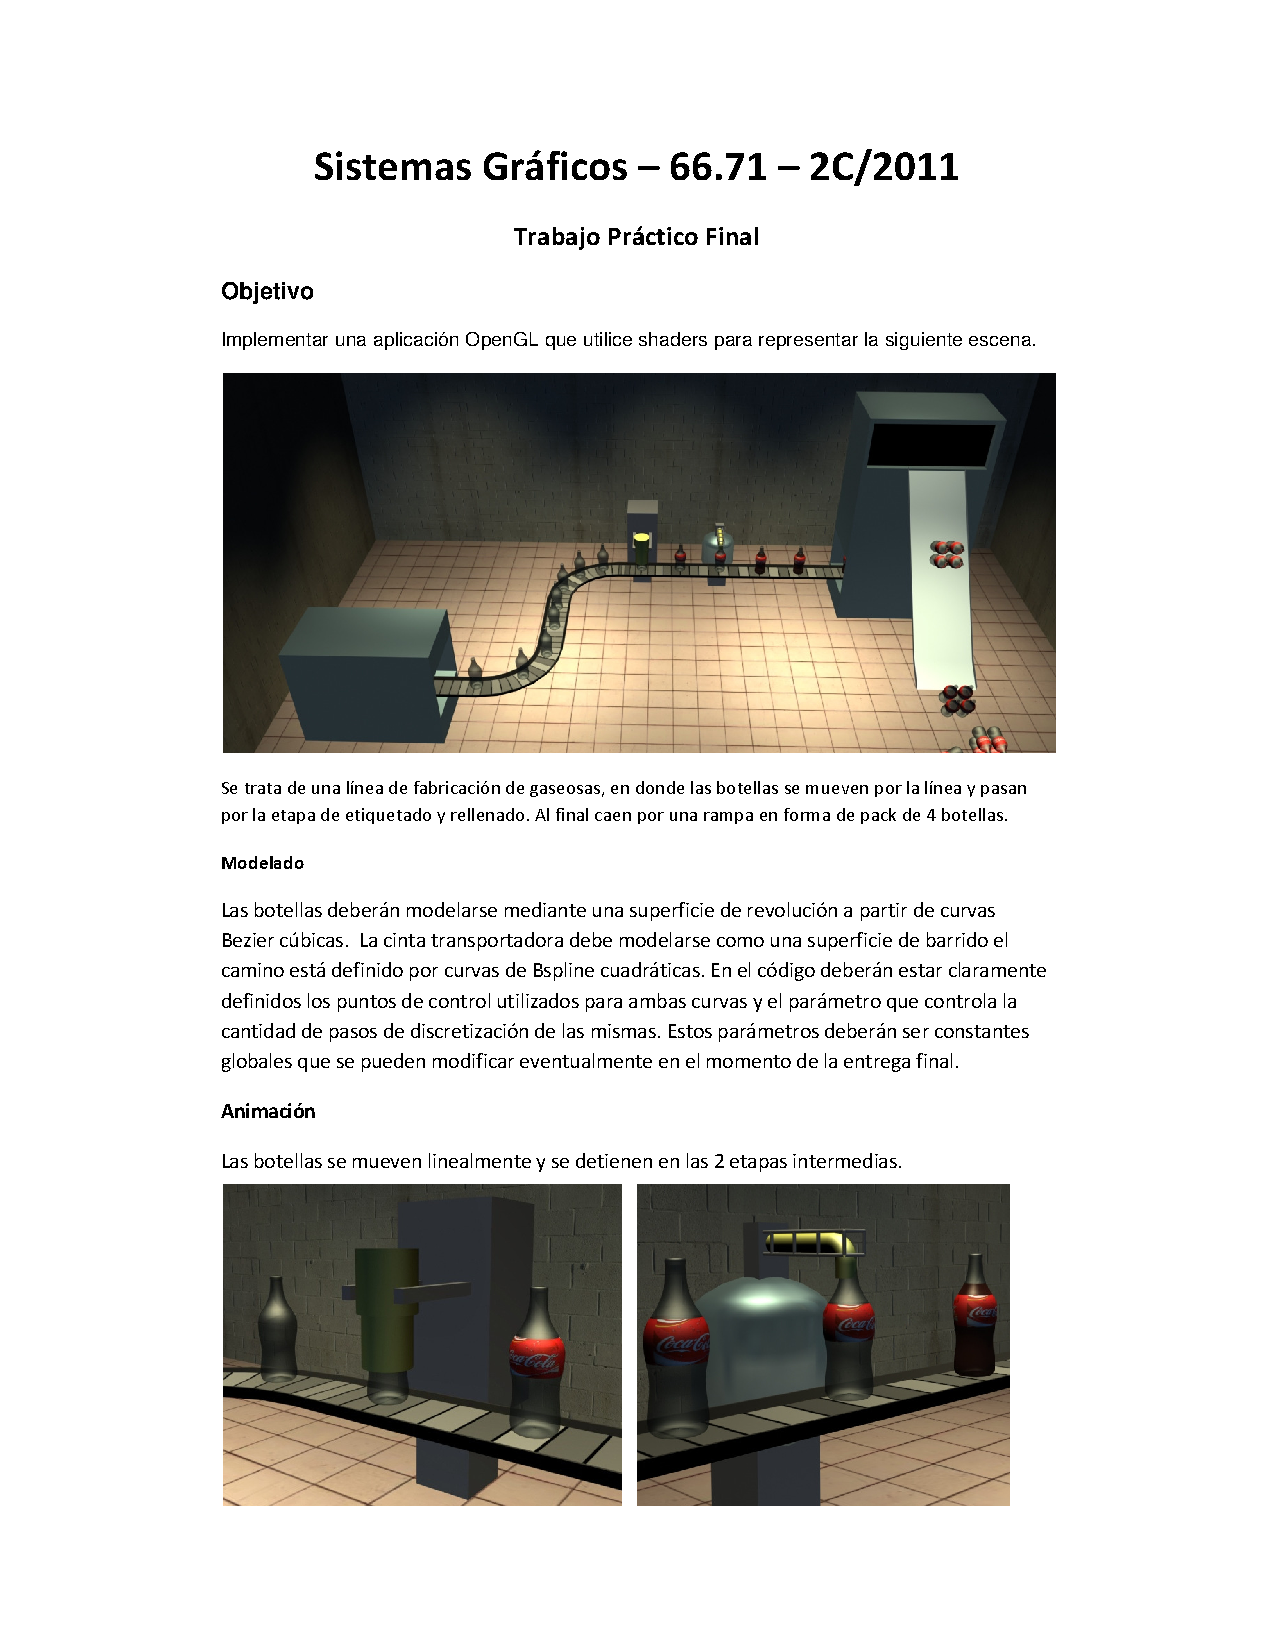
\includegraphics[trim = 25mm 30mm 10mm 35mm, clip,height=0.93\textheight,width=1.04\textwidth]{tpfinal-c2-2011.pdf}
\includegraphics[trim = 25mm 20mm 10mm 25mm, clip,height=0.95\textheight,width=1.04\textwidth,page={2}]{tpfinal-c2-2011.pdf}
\includegraphics[trim = 25mm 20mm 10mm 25mm, clip,height=0.95\textheight,width=1.04\textwidth,page={3}]{tpfinal-c2-2011.pdf}
\includegraphics[trim = 25mm 20mm 10mm 25mm, clip,height=0.95\textheight,width=1.04\textwidth,page={4}]{tpfinal-c2-2011.pdf}
\end{center}

\newpage


\section{Consideraciones de Dise\~no}
Para realizar el presente trabajo pr\'actico se utiliz\'o el lenguaje de programaci\'on GLSL dado que el mismo permite programar la GPU 
de la tarjeta de video para realizar c\'alculos complejos con una mejor performance y precisi\'on.
  Para realizarlo, se tomaron en cuenta las siguientes consideraciones de dise\~no:
\begin{itemize} 
 \item Se debi\'o utilizar la versi\'on 1.2 de GLSL dado que es la soportada por las tarjetas gr\'aficas de las notebooks de la mayor\'ia de 
los integrantes del grupo.
 \item Para el mapeo de texturas en la superficie reflexiva se utiliza un mapa c\'ubico.
 \item Los parámetros tales como los puntos de control de la botella y de la cinta transportadora, los pasos para las curvas y las rotaciones en el
el caso de la superficie de barrido se encuentran definidos en GlobalParameters.h.
\end{itemize}

 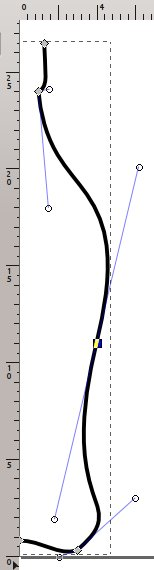
\includegraphics[scale=0.5]{perfil} Perfil de la botella

\subsection{Estructura de la aplicaci\'on}
Para desarrollar la aplicaci\'on se utiliz\'o el lenguaje C++, que permite la programaci\'on orientada a objetos con el encapsulamiento de clases. 
Dentro de las principales, se encuentra la clase TP3; que representa el mundo del trabajo pr\'actico en el cual se suscriben los eventos de OpenGL y responde a las peticiones del usuario. \\\\
Existen shaders de vertices y de fragmentos para:
\begin{itemize} 
 \item La iluminaci\'on basada en los c\'alculos en el modelo de Phong.
 \item La textura y el color de la botella.
 \item La textura cubica necesaria para la superficie reflectiva de la máquina de llenado.
 \item La simulación del avance de la cinta transportadora.
\end{itemize}
\newpage

\section{Compilaci\'on}
  Para compilar la aplicaci\'on bajo entorno Linux se provee un archivo makefile.
  Para utilizar el mismo, debe tenerse instalada la herramienta cmake. Para instalarla, por ejemplo, en una distribuci\'on Ubuntu se deben 
realizar los siguientes pasos: \\
1) sudo apt-get install cmake \\
2) Ingresar la contrase\~na de root del usuario. \\
3) Aceptar la descarga e instalaci\'on de los paquetes necesarios. \\ 

Teniendo ya instalada la herramienta, posicionados en el directorio donde se encuentra el trabajo pr\'actico es necesario crear un directorio build
de la siguiente forma: \\
mkdir build \\
cd build \\
cmake .. \\
make \\

Una vez realizados estos pasos, se dispondr\'a del ejecutable de nombre tp3.

\section{Ejecuci\'on}

Para ejecutar la aplicacio\'n bajo un entorno Linux se deben realizar los siguientes pasos: \\
1)Posicionarse en el directorio build creado anteriormente. \\
2)Ejecutar: \\
./tp3 

\newpage
\section{Controles de teclado}

La aplicaci\'on permite realizar las siguientes acciones utilizando las teclas detalladas a continuaci\'on: \\


    \begin{tabular}{|| l | l ||}
      \hline
      \begin{large}Tecla\end{large} & 
	\begin{large}Acci\'{o}n \end{large} \\
          \hline
x & Rotar la escena con respecto al eje x en el sentido positivo. \\
X & Rotar la escena con respecto al eje x en el sentido negativo. \\
y & Rotar la escena con respecto al eje y en el sentido positivo. \\
Y & Rotar la escena con respecto al eje y en el sentido negativo. \\
z & Rotar la escena con respecto al eje z en el sentido positivo. \\
Z & Rotar la escena con respecto al eje z en el sentido negativo.  \\
+ & Acercar la cámara.  \\
- & Alejar la cámara.  \\
q & Salir de la aplicaci\'on.  \\
r & Resetear la posicion y dirección de la cámara.  \\
e & Activar/desactivar el modo expectador a nivel del suelo para la cámara  \\
S & Pausar/reanudar la simulación.  \\
a & En modo expectador: caminar hacia la izquierda.  \\
d & En modo expectador: caminar hacia la derecha.  \\
s & En modo expectador: caminar hacia atras.  \\
w & En modo expectador: caminar hacia adelante.  \\
          \hline
    \end{tabular}
\\ \\ \\
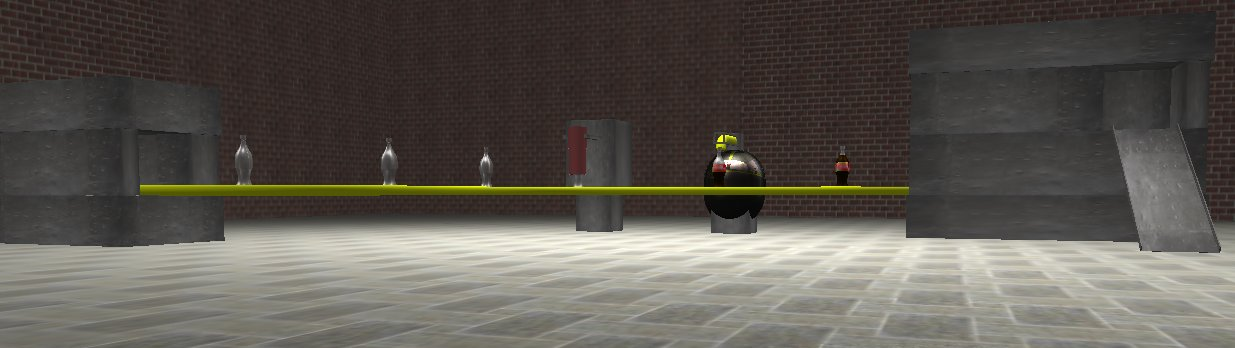
\includegraphics[scale=0.5]{total} \\ Línea de fabricación de gaseosas  \\ \\
 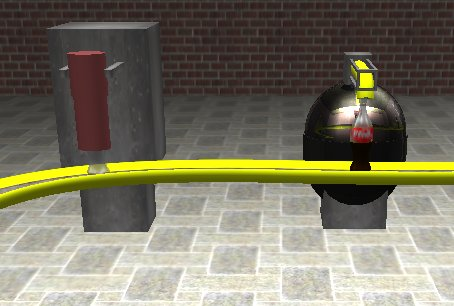
\includegraphics[scale=0.5]{maquinas} Máquina etiquetadora y máquina de llenado \\ \\
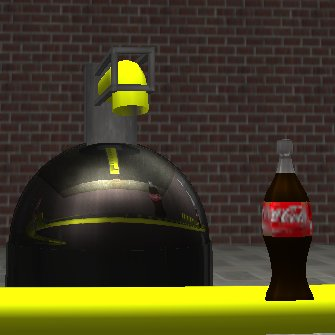
\includegraphics[scale=0.5]{reflejo} Superficie reflectiva de la máquina de llenado \\ \\
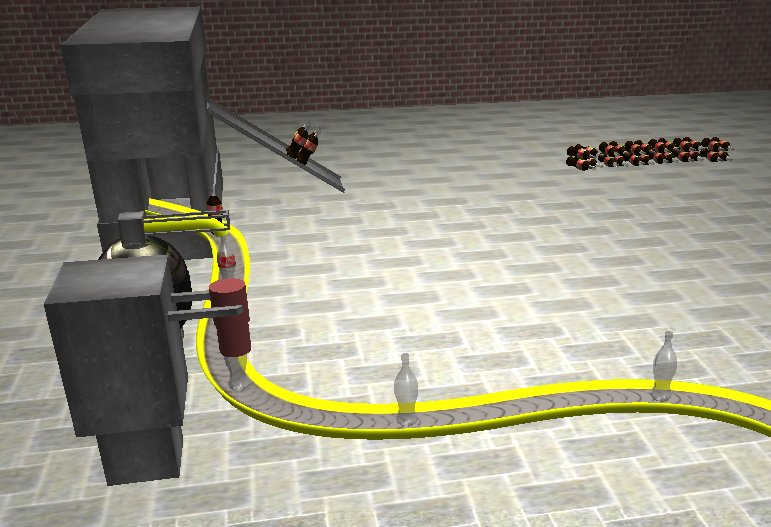
\includegraphics[scale=0.5]{pack1} Packs de botellas

\end{document}

